\section{Quadraturas de Gauss}

\subsection{Quadraturas de Gauss-Legendre}

\begin{enumerate}

\item 
OBS:

\begin{enumerate}

\item 
S\~ao m\'etodos num\'ericos de integra\'c\~ao que utilizam os pontos de Legendre (ra\'izes dos polin\^omios de Legendre)

\item
Apropriadas para fun\'c\~oes anal\'iticas.

\item
Precis\~ao muito maior do que as f\'ormulas de Newton-Cotes.

\item
Os pontos de Legendre \textbf{não são regularmente espaçados.}

\end{enumerate}

\item

\begin{enumerate}

 \item 
Erro da Regra do Trap\'ezio \'e proporcional a $f''$. Assim, se $f(x)$ for polin\^omio at\'e ordem 1, o erro \'e nulo.

\item
Erro da Regra do Trapézio é proporcional a $f^{IV}$. Assim, integra exatamente polinômios de até ordem 3.

\item
As fórmulas de Newton-Cotes com $n$ ímpar integram exatamente polinômios de ordem $n$ e as com $n$ par integram exatamente polinômios de ordem $n+1$.

\item
Vamos tentar uma fórmula de integração com dois pontos que integre exatamente um polinômio de ordem 3 (3 pontos [N-Cotes $n=2$] ou 4 pontos [N-Cotes $n=3$]).

\end{enumerate}

\begin{equation}
 \label{cap2:sec6:eq1}
 I = \int_{-1}^1 f\,(x) \, dx = w_1 \, f\,(x_1) + w_2 \, f\,(x_2) + E
\end{equation}

Queremos $E=0$ para $f(x)=1$, $f(x)=x$, $f(x)=x^{2}$ e $f(x)=x^{3}$.

Assim,

\begin{equation}
 \label{cap2:sec6:eq2}
 \begin{array}{llr}
  \int_{-1}^1 1 \, dx & = 2 = w_1 + w_2 \qquad & (a) \\
  \int_{-1}^1 x \, dx & = 0 = w_1\,x_1 + w_2\,x_2 \qquad & (b) \\
  \int_{-1}^1 x^2 \, dx & = \displaystyle \frac{2}{3} = w_1\,x_1^2 + w_2\,x_2^2 \qquad & (c) \\
  \int_{-1}^1 x^3 \, dx & = 0 = w_1\,x_1^3 + w_2\,x_2^3 \qquad & (d)
 \end{array}
\end{equation}

os limites de integração são simétricos em relação a $x=?$.

Assim, façamos $x_{1}$ e $x_{2}$ simétricos em relação a $x=0$

\[x_{2} = -x_{1}\]

\[
 \begin{array}{l}
  (\ref{cap2:sec6:eq2}.b) \Rightarrow w_1\,x_1 - w_2\,x_1 = x_1\,(w_1 - w_2) = 0 \\
  (\ref{cap2:sec6:eq2}.a) \Rightarrow w_1 + w_2 = 2 \neq 0 \Rightarrow w_1 = w_2 = 1
 \end{array}
\]

Com estes valores (\ref{cap2:sec6:eq2}.d) fica automaticamente satisfeita

\[
 0 = 1\,x_1^3 + 1\,(-x_1)^3 = x_1^3 - x_1^3
\]

\[
 \begin{array}{l}
  (\ref{cap2:sec6:eq2}.c) \Rightarrow \displaystyle \frac{2}{3} = x_1^2 + (-x_1)^2 = 2\,x_1^2 \Rightarrow x_1^2 = \frac{1}{3} \\ \\
  \qquad x_1 = \displaystyle \frac{1}{\sqrt{3}} \vspace*{0.2cm} \\
  \qquad x_2 = - \displaystyle \frac{1}{\sqrt{3}}
 \end{array}
\]


Para $n$ pontos de integração $x_{1}$, $x_{2}$, ... $x_{n}$ são as raízes do polinômio de Legendre de ordem $n$.

\[
 \quadricular{\displaystyle \int_{-1}^1 f\,(x) \, dx \approx \sum_{k=1}^N w_k \, f\,(x_k)}
\]

Polinômio de Legendre de ordem $n$.

\[
 P_n\,(x) = \frac{1}{2^N\,N!} \, \frac{d^N\,(x^2 - 1)^N}{dx^N}
\]

\[
 \begin{array}{l}
  P_0\,(x) = \displaystyle \frac{1}{2^0\,0!} \, (x^2 - 1)^0 = 1 \vspace*{0.2cm} \\
  P_1\,(x) = \displaystyle \frac{1}{2^1\,1!} \, \frac{d}{dx} \, (x^2 - 1)^1 = x \vspace*{0.2cm} \\
  P_2\,(x) = \displaystyle \frac{1}{2^2\,2!} \, \frac{d^2}{dx^2} \, (x^2 - 1)^2 = \frac{1}{2}\,(3\,x^2 - 1)
 \end{array}
\]

\begin{table}[htp]
\footnotesize
	\centering
		
		\begin{tabular}{|ccc|}
		\hline		
		& \textbf{$\pm \, x_i$} & \textbf{$w_i$} \\
		\hline \hline
		N=2 & $\pm$ 0.577350269 & 1.0 \\
		\hline 
		N=3 &
		$
		\left\{
		\begin{array}{l}
		 0 \\
		 \pm 0.774596669
		\end{array}
		\right.
		$
		&
		$
		\begin{array}{l}
		 0.888888889 = 8/9 \\
		 0.555555556 = 5/9
		\end{array}
		$
		\\
		\hline 
		N=4 &
		$
		\left\{
		\begin{array}{l}
		 \pm 0.339981043 \\
		 \pm 0.861136312
		\end{array}
		\right.
		$
		&
		$
		\begin{array}{l}
		 0.652145155 \\
		 0.347854845
		\end{array}
		$
		\\
		\hline
		\vdots & \vdots & \vdots \\
		\hline
		\end{tabular}
	%\caption{}
	\label{cap2:sec5:tab1}
\end{table}

\[
 \begin{array}{ll}
  I & = \displaystyle \int_a^b \, f\,(x) \, dx = \\ \\
    & = \displaystyle \frac{b-a}{2} \, \int_{-1}^1 \bar{f}\,(\xi) \, d\xi \\ \\
    & = \displaystyle \frac{b-a}{2} \, \sum_{k=1}^N \, w_k \, \bar{f}\,(\xi_k)
 \end{array}
\]

\begin{figure}[htb]
 \centering
 \begin{minipage}[c]{7cm}
    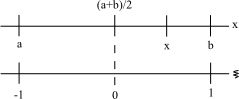
\includegraphics[scale=0.8]{capitulos/capitulo2/figuras/quadraturas_de_gauss1.png}
    \caption{Parametrização}
    \label{fig:quadraturas_de_gauss1}
 \end{minipage}\hspace*{1cm}
 \begin{minipage}[c]{6cm}
     \[
      \begin{array}{ll}
       x & = \displaystyle \frac{a+b}{2} + \xi \, \left(\frac{b-a}{2}\right) \\
       dx & = \displaystyle \frac{b-a}{2} \, d\xi
      \end{array}
     \]
 \end{minipage}
\end{figure}

\begin{example}
\[
 I = \int_0^2 \, \pi \, [1 + (x/2)^2]^2 \, dx
\]

\[
 \begin{array}{lll}
 \left.
 \begin{array}{l}
  b = 2 \\
  a = 0
 \end{array}
 \right\}
 & x & = \displaystyle \frac{0+2}{2} + \displaystyle \frac{2-0}{2} \, \xi = 1 + \xi \Rightarrow x = 1 + \xi \\
 & dx & = d\xi
 \end{array}
\]

$n=2$ integra exatamente $2n-1 = 4-1 = 3$

$n=3$ integra exatamente polinômio de grau $\leq$ 5.

Como o integrando é polinômio de grau 4 utilizaremos $n=3$

\[
\begin{array}{l}
 \xi_1 = - 0.774596669 \rightarrow f_1 = \pi \, \left\{ 1 + \left[ (1+\xi_1)/2 \right]^2 \right\}^2 = 3.2219064 \qquad w_1=5/9 \\
 ?
\end{array}
\]

\[
\begin{array}{ll}
 I & = \displaystyle \frac{5}{9} \, 3.2219064 + \frac{8}{9} \, 4.9087385 + \frac{5}{9} \, 10.0356146 \\
   & = 11.7286
\end{array}
\]

\end{example}

\item
Provar que, se $f(x)$ for um polinômio de ordem $2n-1$ ou menor, a quadratura de Gauss de ordem $n$ é exata.

\textbf{Prova:} Suponha que $f(x)$ em \esp{\int_{-1}^1 \, f\,(x) \, dx} seja um polinômio de ordem $2n-1$. Assim,

\begin{equation}
 \label{cap2:sec6:eq1}
 f\,(x) = c\,(x) \, P_N\,(x) + r\,(x)
\end{equation}

onde $P_{n}(x)$ é o polinômio de Legendre de ordem $n-1$

\begin{equation}
 \label{cap2:sec6:eq2}
 \int_{-1}^1 \, f\,(x)\,dx = \underbrace{\int_{-1}^1 \, c\,(x)\,P_N\,(x)\,dx}_{
  \begin{array}{l}
   \mbox{\footnotesize{$= 0$, pois o polinômio $P_N$}} \\
   \mbox{\footnotesize{é ortogonal a todos os}} \\
   \mbox{\footnotesize{polinômios de ordem $< N-1$}}
  \end{array}
 } + \int_{-1}^1 \, r\,(x)\,dx
\end{equation}

\begin{equation}
 \underbrace{
 \quadricular{
 \label{cap2:sec6:eq3}
 \int_{-1}^1 \, P_m \, (x) \, dx =
 \left\{
  \begin{array}{cl}
   0 & \qquad \mbox{para } n \neq m \\ \\
   \displaystyle \frac{2}{2\,n+1} & \qquad \mbox{para } m = n
  \end{array}
 \right.
 }
 }_{
  \mbox{\footnotesize{ortogonalidade dos polinômios de Legendre}}
 }
\end{equation}

\begin{equation}
 \label{cap2:sec6:eq4}
 \int_{-1}^1 \, f\,(x) \, dx = \int_{-1}^1 \, r\,(x) \, dx 
\end{equation}

Se $x_{i}$ é uma das raízes do polinômio de Legendre $P_{n}$, então:

\begin{equation}
 \label{cap2:sec6:eq5}
 f\,(x_i) = \underbrace{c\,(x_i) \, P_n\,(x_i)}_{0} + \, r\,(x_i) \Rightarrow f\,(x_i) = r\,(x_i)
\end{equation}

O polinômio \esp{r\,(x)} de ordem \esp{N-1} pode ser expresso exatamente pela interpolação de Lagrange de ordem \esp{N-1} (precisa de \esp{N} pontos amostrais)

\begin{equation}
 \label{cap2:sec6:eq6}
 r\,(x) =
 \sum_{i=1}^N \left[
  \prod_{
    j=1 \,\, j \neq i
  }^N
  \frac{x-x_j}{x_i-x_j}
 \right]
 r\,(x_i)
\end{equation}

\begin{example}

\begin{figure}[htb]
 \centering
 \begin{minipage}[c]{7cm}
    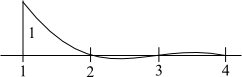
\includegraphics[scale=0.9]{capitulos/capitulo2/figuras/quadraturas_de_gauss2.png}
    \caption{?}
    \label{fig:quadraturas_de_gauss2}
 \end{minipage}\hspace*{1cm}
 \begin{minipage}[c]{6cm}
    \[
     r_1 \, \frac{x-x_2}{x_1-x_2} \, \frac{x-x_3}{x_1-x_3} \, \frac{x-x_4}{x_1-x_4}
    \]
 \end{minipage}
\end{figure}

\begin{figure}[htb]
 \centering
 \begin{minipage}[c]{7cm}
    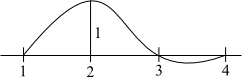
\includegraphics[scale=0.9]{capitulos/capitulo2/figuras/quadraturas_de_gauss3.png}
    \caption{?}
    \label{fig:quadraturas_de_gauss3}
 \end{minipage}\hspace*{1cm}
 \begin{minipage}[c]{6cm}
    \[
     r_2 \, \frac{x-x_1}{x_2-x_1} \, \frac{x-x_3}{x_2-x_3} \, \frac{x-x_4}{x_2-x_4}
    \]
 \end{minipage}
\end{figure}

\begin{figure}[htb]
 \centering
 \begin{minipage}[c]{7cm}
    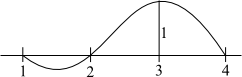
\includegraphics[scale=0.9]{capitulos/capitulo2/figuras/quadraturas_de_gauss4.png}
    \caption{?}
    \label{fig:quadraturas_de_gauss4}
 \end{minipage}\hspace*{1cm}
 \begin{minipage}[c]{6cm}
    \[
     r_3 \, \frac{x-x_1}{x_3-x_1} \, \frac{x-x_2}{x_3-x_2} \, \frac{x-x_4}{x_3-x_4}
    \]
 \end{minipage}
\end{figure}

\begin{figure}[htb]
 \centering
 \begin{minipage}[c]{7cm}
    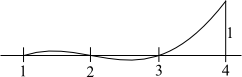
\includegraphics[scale=0.9]{capitulos/capitulo2/figuras/quadraturas_de_gauss5.png}
    \caption{?}
    \label{fig:quadraturas_de_gauss5}
 \end{minipage}\hspace*{1cm}
 \begin{minipage}[c]{6cm}
    \[
     r_4 \, \frac{x-x_1}{x_4-x_1} \, \frac{x-x_2}{x_4-x_2} \, \frac{x-x_3}{x_4-x_3}
    \]
 \end{minipage}
\end{figure}

\end{example}

Se os pontos amostrais forem as \esp{N} raízes de \esp{P_N\,(x)}, então, pela equação \ref{cap2:sec6:eq5}

\begin{equation}
 \label{cap2:sec6:eq7}
 r\,(x) =
 \sum_{i=1}^N \left[
  \prod_{
    j=1 \,\, j \neq i
  }^N
  \frac{x-x_j}{x_i-x_j}
 \right]
 f\,(x_i)
\end{equation}

Assim \ref{cap2:sec6:eq7} $\rightarrow$ \ref{cap2:sec6:eq4} $\Rightarrow$

\[
 \int_{-1}^1 \, f\,(x) \, dx = \int_{-1}^1 \, r\,(x) \, dx = \sum_{i=1}^N \, f\,(x_i) \,
 \underbrace{
 \int_{-1}^1 \left[
  \prod_{
    j=1 \,\, j \neq i
  }^N
  \frac{x-x_j}{x_i-x_j}
 \right]
 \, dx
 }_{
  w_i
 }
\]
\begin{example}
 \emph{ Deducao de Quadraturas de Gauss-legendre } 

-

-

A quadratura de Gauss-legendre é dada pela fórmula (4.6.1, na página
135 do livro Applied Numerical methods, Nakamura)

Temos que:

\emph{\[
\int_{-1}^{1}{\scriptstyle f(x)dx}\backsimeq\sum_{{\scriptstyle {\scriptscriptstyle k=1}}}^{{\scriptscriptstyle N}}{\scriptstyle w_{k}f(x_{k})}\]
}

Onde$x_{1},x_{2},x_{3}...x_{n}$ é dado pelas raizes de $P_{N}(x)=0$,$P_{N}(x)$
é o Polinomio de Legendre de ordem N. Tal polinomio é dado pela seguinte
fórmula(Appendix B, página 559 do livro Applied Numerical Methods,
Nakamura): \[
P_{4}(x)=\frac{1}{2^{4}4!}\frac{d^{4}(x^{2}-1)^{4}}{dx^{4}}\]


Onde, 

\[
\frac{1}{2^{4}4!}=\frac{1}{384}\]


logo, teremos:

\[
\frac{1}{384}\frac{d^{4}(x^{2}-1)^{4}}{dx^{4}}=\frac{1}{384}\frac{d^{4}}{dx^{4}}(x^{8}-4x^{6}+6x^{4}-4x^{2}+1)=\frac{1}{8}(35x^{4}-30x^{2}+3)\]


Para tirarmos as raízes, temos que:

\[
P_{4}(x)=0\]


Então,

\[
(35x^{4}-30x^{2}+3)=0\]


Tirando as raízes:

%\lyxline{\normalsize}

$x^{2}=a$ ,então a fórmula se tornará , $35a^{2}-30a+3=0$, daqui
é fácil ver que as raízes de a são: $a_{1}=\frac{15+2\sqrt{30}}{35}$
e $a_{2}=\frac{15-2\sqrt{30}}{35}$ .

como $x^{2}=a$ , teremos: $x_{1}=\sqrt{\frac{15+2\sqrt{30}}{35}};x_{2}=-\sqrt{\frac{15+2\sqrt{30}}{35}};x_{3}=\sqrt{\frac{15-2\sqrt{30}}{35}};x_{4}=-\sqrt{\frac{15-2\sqrt{30}}{35}};$

Teremos, então, $x_{1}=0,861136312;x_{2}=-0,861136312;x_{3}=0,339981043;x_{4}=-0,339981043;$

%\lyxline{\normalsize}

Como os pontos devem ser localizados simetricamente, temos que: $w_{1}=w_{2}$e$w_{3}=w_{4}.$

O cálculo de w é dado pela fórmula(página 138, do livro Applied Numerical
methods, Nakamura):

\[
w_{i}=\int_{-1}^{1}\left[\prod_{{\scriptscriptstyle j=1;j\neq i}}^{{\scriptscriptstyle N}}{\scriptstyle \frac{{\scriptstyle x-x_{j}}}{x_{i}-x_{j}}}\right]dx\]


Para $w_{1}$, teremos:

\[
w_{1}=\int_{-1}^{1}\left[\prod_{{\scriptscriptstyle j=1;j\neq i}}^{{\scriptscriptstyle N}}{\scriptstyle \frac{{\scriptstyle x-x_{j}}}{x_{i}-x_{j}}}\right]dx=\int_{-1}^{1}\left[\frac{(x-x_{2})(x-x_{3})(x-x_{4})}{(x_{1}-x_{2})(x_{1}-x_{3})(x_{1}-x_{4})}\right]dx\]


Integrando, temos:

\[
w_{1}=w_{2}=0,347854845\]


E para $w_{3}$, teremos:

\[
w_{3}=\int_{-1}^{1}\left[\prod_{{\scriptscriptstyle j=1;j\neq i}}^{{\scriptscriptstyle N}}{\scriptstyle \frac{{\scriptstyle x-x_{j}}}{x_{i}-x_{j}}}\right]dx=\int_{-1}^{1}\left[\frac{(x-x_{1})(x-x_{2})(x-x_{4})}{(x_{3}-x_{1})(x_{3}-x_{2})(x_{3}-x_{4})}\right]dx\]


Após integrar, teremos:

Temos, então:

\[
w_{3}=w_{4}=0,652145155\]


Substituindo os resultados, na fórmula da quadratura de Gauss-legendre
aplicada a N=4, teremos:

\[
\int_{-1}^{1}{\scriptstyle f(x)dx}\backsimeq0,347854845f(0,861136312)+0,347854845f(-0,861136312)\]


\[
+0,652145155f(0,339981043)+0,652145155f(-0,339981043)_{\blacksquare}\]
\end{example}


\subsection{Outras Quadraturas de Gauss}

\begin{enumerate}

\item 
\textbf{Gauss-Hermite}: apropriadas para integrais da forma

\[
 I = \int_{-\infty}^\infty \, e^{-x^2} \, f\,(x) \, dx \approx \sum_{k=1}^N \, w_k \, f\,(x_k)
\]

{
%\begin{table}[htp]
\footnotesize
	\begin{center}
		\begin{tabular}{|c|c|c|}
		\hline		
		\textbf{N} & \textbf{Pontos de Hermite: $\pm \, x_i$} & \textbf{Pesos de Hermite: $w_i$} \\
		\hline \hline
		2 & $\pm 0.70710678$ & $0.88622692$ \\
		\hline
		3 & $0.00000000$     & $1.18163590$ \\
		  & $\pm 1.22474487$ & $0.29540897$ \\
		\hline
		4 & $\pm 0.52464762$ & $0.80491409$ \\
		  & $\pm 1.65068012$ & $0.08131283$ \\
		\hline
		5 & $    0.00000000$ & $0.94530872$ \\
		  & $\pm 0.95857246$ & $0.39361932$ \\
		  & $\pm 2.02018287$ & $0.01995324$ \\
		\hline
		\end{tabular}
	\end{center}
	\label{cap2:sec6:tab2}
%\end{table}
}

\item
\textbf{Gauss-Laguerre}: apropriadas para integrais da forma

\[
 I = \int_0^\infty \, e^{-x} \, f\,(x) \, dx \approx \sum_{k=1}^N \, w_k \, f\,(x_k)
\]

{
%\begin{table}[htp]
\footnotesize
	\begin{center}
		\begin{tabular}{|c|c|c|}
		\hline		
		\textbf{N} & \textbf{Pontos de Laguerre: $x_i$} & \textbf{Pesos de Laguerre: $w_i$} \\
		\hline \hline
		2 & $0.58578643$ & $0.85355339$ \\
		  & $3.41421356$ & $0.14644660$ \\
		\hline
		3 & $0.41577455$ & $0.71109300$ \\
		  & $2.24428036$ & $0.27851973$ \\
		  & $6.28994508$ & $0.01038926$ \\
		\hline
		4 & $0.32254768$ & $0.60315410$ \\
		  & $1.74576110$ & $0.35741869$ \\
		  & $4.53662029$ & $0.03888791$ \\
		  & $9.39507091$ & $0.00053929$ \\
		\hline
		\end{tabular}
	\end{center}
	\label{cap2:sec6:tab3}
%\end{table}
}

\item
\textbf{Gauss-Chebyshev}: apropriadas para integrais da forma

\[
 I = \int_{-1}^1 \, \frac{1}{\sqrt{1-x^2}} \, f\,(x) \, dx \approx \sum_{k=1}^N \, w_k \, f\,(x_k)
\]

onde \esp{x_k = \cos\,\frac{k-1/2}{N} \, \pi}, \esp{k=1, 2, \ldots, N}

\[
 w_k = \frac{\pi}{N} \qquad \forall k
\]

Assim,

\[
 I = \int_{-1}^1 \, \frac{1}{\sqrt{1-x^2}} \, f\,(x) \, dx \approx \frac{\pi}{N} \, \sum_{k=1}^N \, f\,(x_k)
\]

\end{enumerate}

\end{enumerate}

\textbf{Nota}: todas as três quadraturas serão exatas se $f(x)$ for um polinômio de ordem $\leq 2n-1$ 